\section{Evaluation}

We evaluate the system on two complementary axes: (i) quantitative knowledge retention on the MINE-1 benchmark~\citep{mo2025kggen} against KGGen, GraphRAG, and OpenIE; and (ii) qualitative multi-standard analysis across three Trustworthy AI regulatory documents addressing RQ1--RQ4.

\subsection{Experimental Setup}

\textbf{Backbone LLM.} All extraction stages use an OpenAI-compatible endpoint serving \texttt{deepseek-r1:32b} (on-premise DFKI infrastructure). The same judge model is used for novelty classification (temperature 0.0) and conflict judgment (temperature 0.0).

\textbf{Encoder.} All embedding operations use \texttt{all-MiniLM-L6-v2} (SentenceTransformers; 22.7M parameters). This model is held constant across all compared systems in the MINE-1 evaluation.

\textbf{Standards corpus.} For multi-standard analysis, we ingest three documents: (i) EU AI Act Article 10 (Data and Data Governance provisions)~\citep{euAIAct2024}; (ii) ISO/IEC 42001:2023 (AI Management Systems)~\citep{iso42001}; and (iii) ISO/IEC 5259-3 (Data Quality for Analytics and ML)~\citep{iso52593}. All documents address the data governance and quality dimensions of Trustworthy AI.

\subsection{RQ1: Knowledge Retention (MINE-1 Benchmark)}

\textbf{Benchmark.} MINE-1~\citep{mo2025kggen} evaluates the knowledge retention of a KG by checking whether 15 known facts per article can be recovered from the graph via a fixed retrieval-judge pipeline. The benchmark comprises 100 short general-knowledge articles. For each fact, a retriever (\texttt{all-MiniLM-L6-v2}, top-$k$ nearest nodes + 2-hop expansion) pulls a context subgraph, and an LLM judge assigns a binary recovered/not-recovered verdict. MINE-1 = \% of facts scored as recovered, averaged over all 100 articles. Retriever and judge are held constant across all systems; the benchmark therefore isolates \emph{graph-content quality}.

\textbf{MINE mode.} Because the controlled predicate vocabulary is calibrated for regulatory text, we run KBDebugger in MINE mode for this evaluation: keyword gate disabled (full document extraction), similarity and novelty filters disabled, and triplet extraction using a free-form predicate prompt (\texttt{neutral\_mode=True}) comparable to KGGen's output format. This ensures a fair comparison of extraction \emph{core quality}, not vocabulary fit.

\textbf{Results.} Table~\ref{tab:mine1} shows MINE-1 scores across systems and judges.

\begin{table}[t]
\centering
\caption{MINE-1 Knowledge Retention. Our system vs.\ published baselines (KGGen, GraphRAG, OpenIE). Retriever fixed to \texttt{all-MiniLM-L6-v2}; judge columns show different LLM judges. $\dagger$: published baseline from~\citet{mo2025kggen} (GPT-4o/Gemini backbone). $\ddagger$: re-evaluated under our judge on-premise.}
\label{tab:mine1}
\begin{tabularx}{\columnwidth}{lXXX}
\toprule
\textbf{System} & \textbf{DeepSeek-R1} & \textbf{GPT-5 (top-10)} & \textbf{Qwen3-30B} \\
\midrule
OpenIE$^\dagger$        & 52.3\% & --     & --     \\
GraphRAG$^\dagger$      & 58.1\% & --     & --     \\
KGGen$^\dagger$         & 62.7\% & 62.9\% & 75.4\% \\
\midrule
\textbf{Ours}$^\ddagger$ & \textbf{79.4\%} & \textbf{79.3\%} & \textbf{92.9\%} \\
\bottomrule
\end{tabularx}
\end{table}

Our system achieves 79.4\% under the DeepSeek-R1 judge (+16.7~pp over KGGen), 79.3\% under GPT-5 on the top-10 articles, and 92.9\% under Qwen3-30B. The consistent ranking across three independent judges confirms that the improvement reflects actual graph-content quality, not judge-specific scoring artifacts. Figure~\ref{fig:mine_dist} shows the per-article score distributions for our system and KGGen under DeepSeek-R1.

\begin{figure}[t]
    \centering
    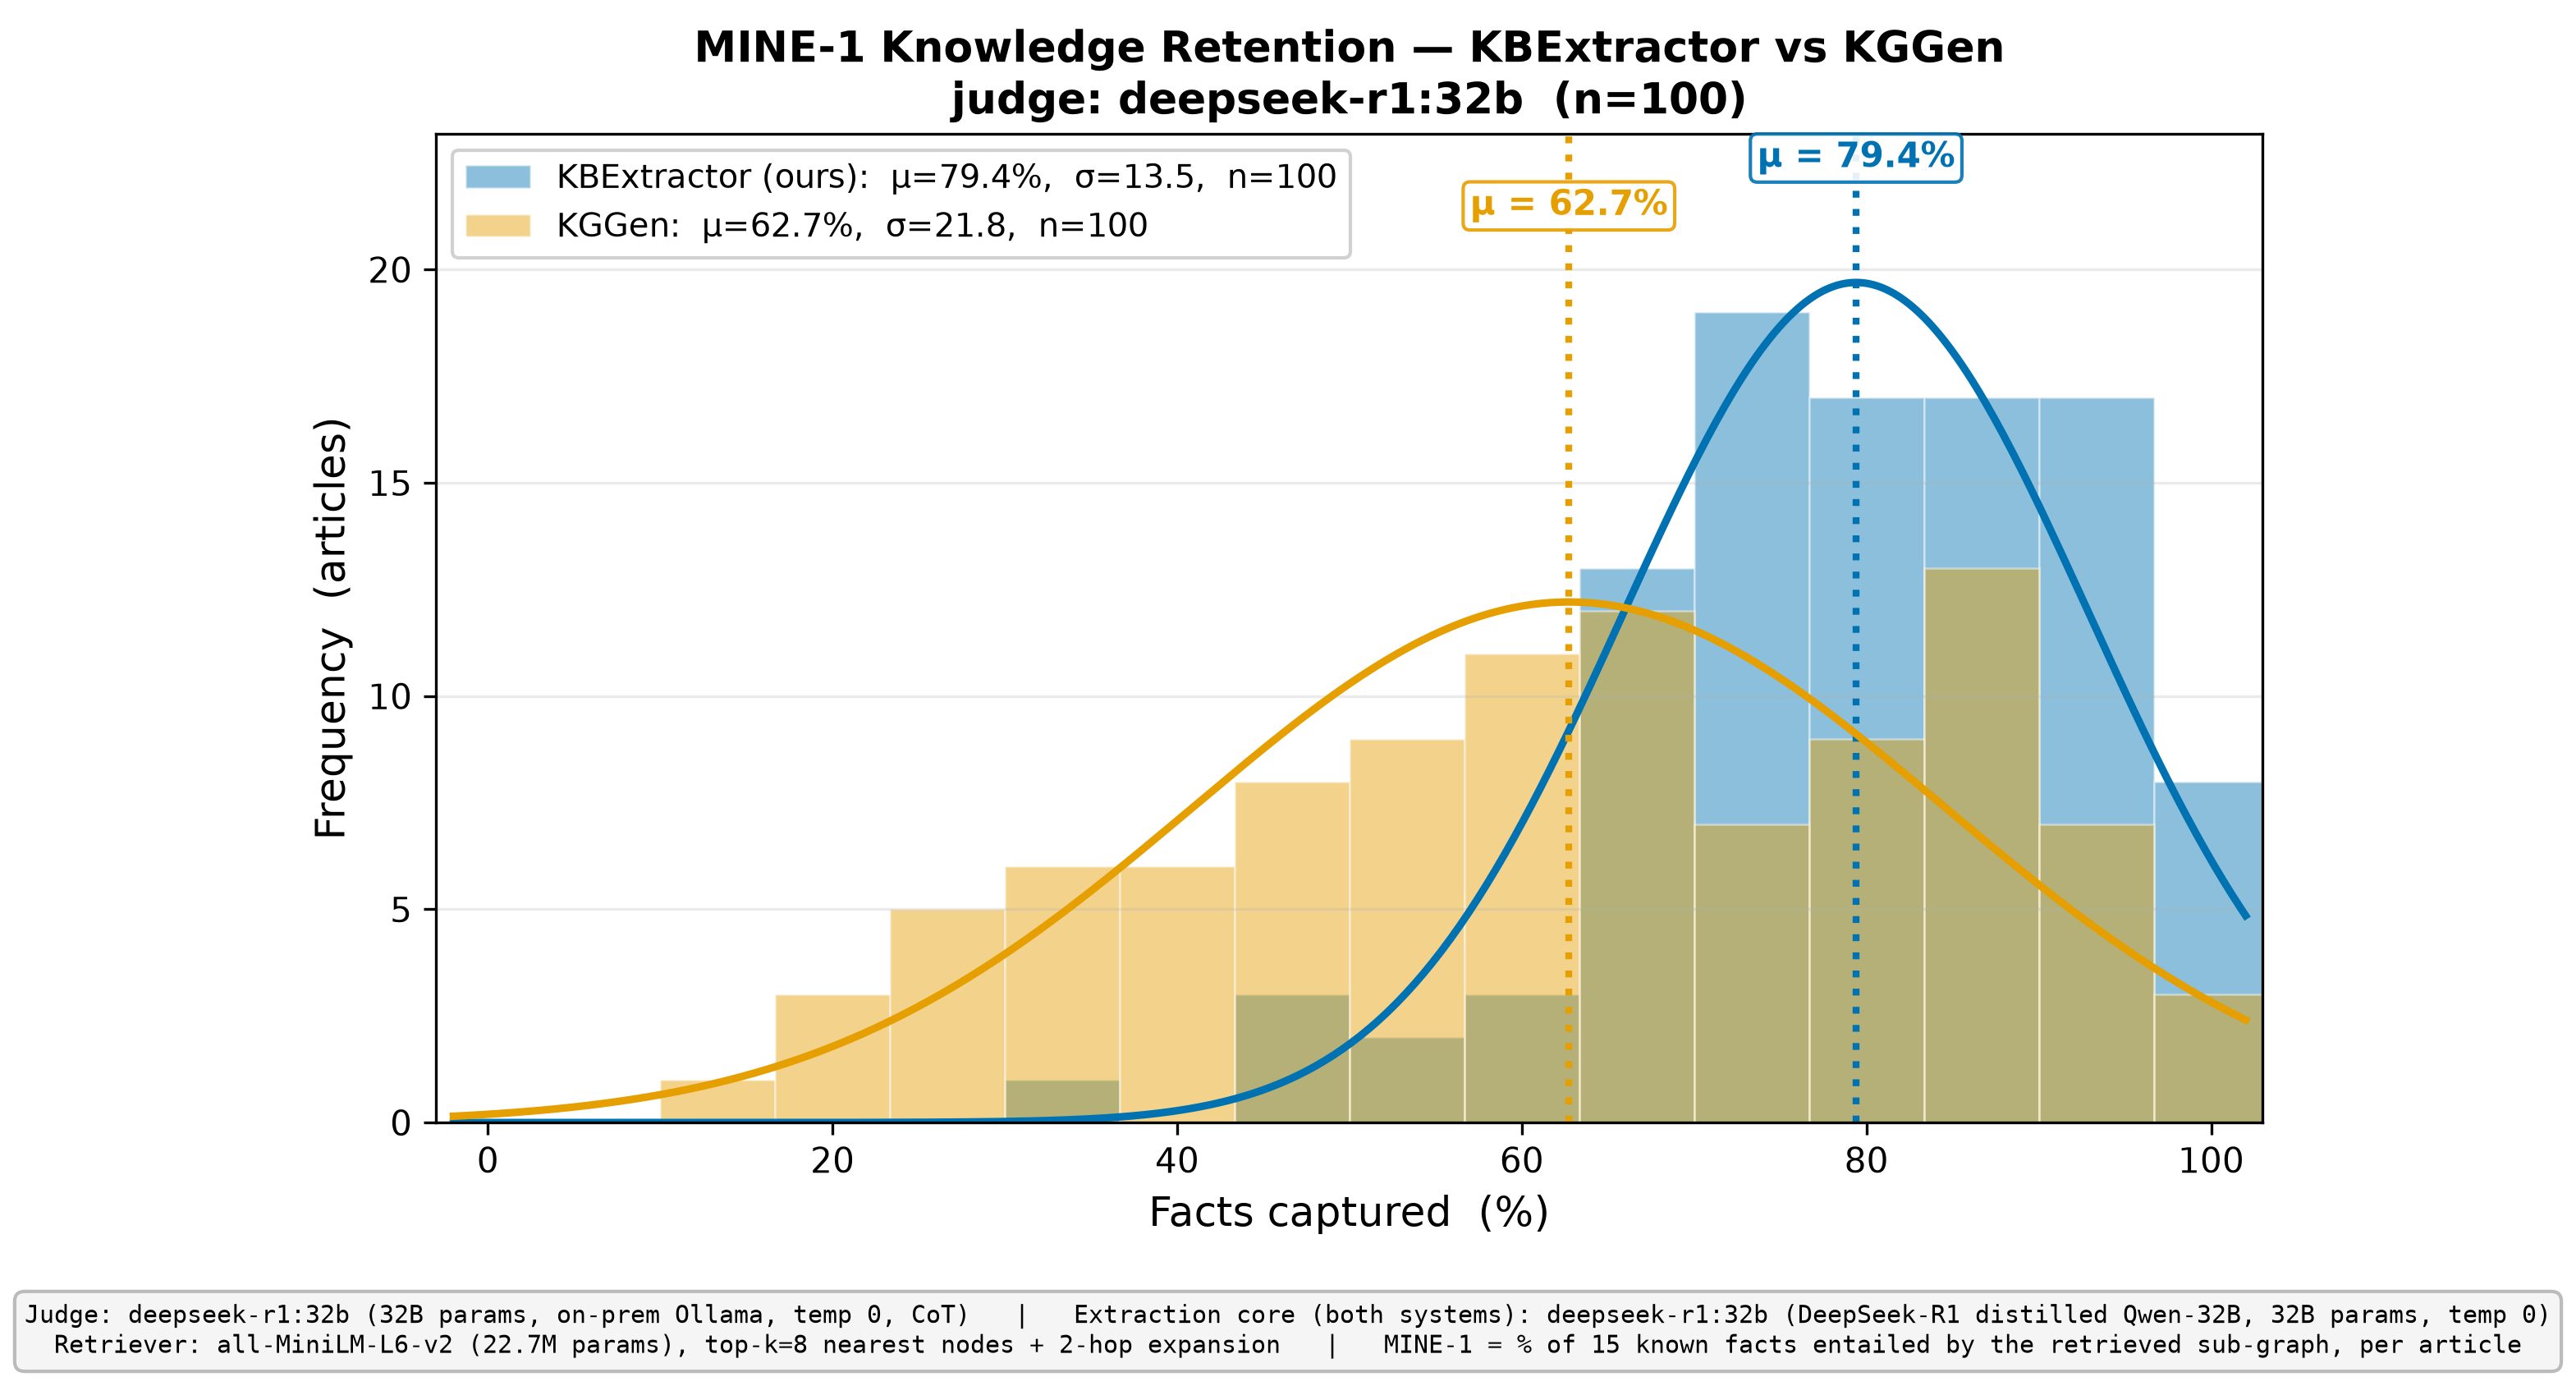
\includegraphics[width=\columnwidth]{Figures/mine/mine1_distribution_deepseek.png}
    \caption{MINE-1 per-article score distribution for our system (blue) and KGGen (orange) under the DeepSeek-R1 judge. Our system produces fewer low-scoring articles and a heavier right tail, consistent with its higher decomposition granularity.}
    \label{fig:mine_dist}
\end{figure}

\textbf{Why does decomposition help?} We attribute the improvement primarily to atomic quality decomposition (Stage 2c): by splitting compound sentences before triplet extraction, each retained fact is more likely to surface as a standalone triple. In contrast, KGGen operates on full sentences, which causes semantically distinct facts embedded in the same sentence to be collapsed into a single, coarser triple. This is corroborated by Figure~\ref{fig:mine_paired}, which shows a paired article-level comparison: our system outperforms KGGen on 67 of 100 articles. The article-level advantage is statistically robust (sign test: $p < 0.001$), confirming the overall gain is not driven by a small number of high-scoring outliers.

\begin{figure}[t]
    \centering
    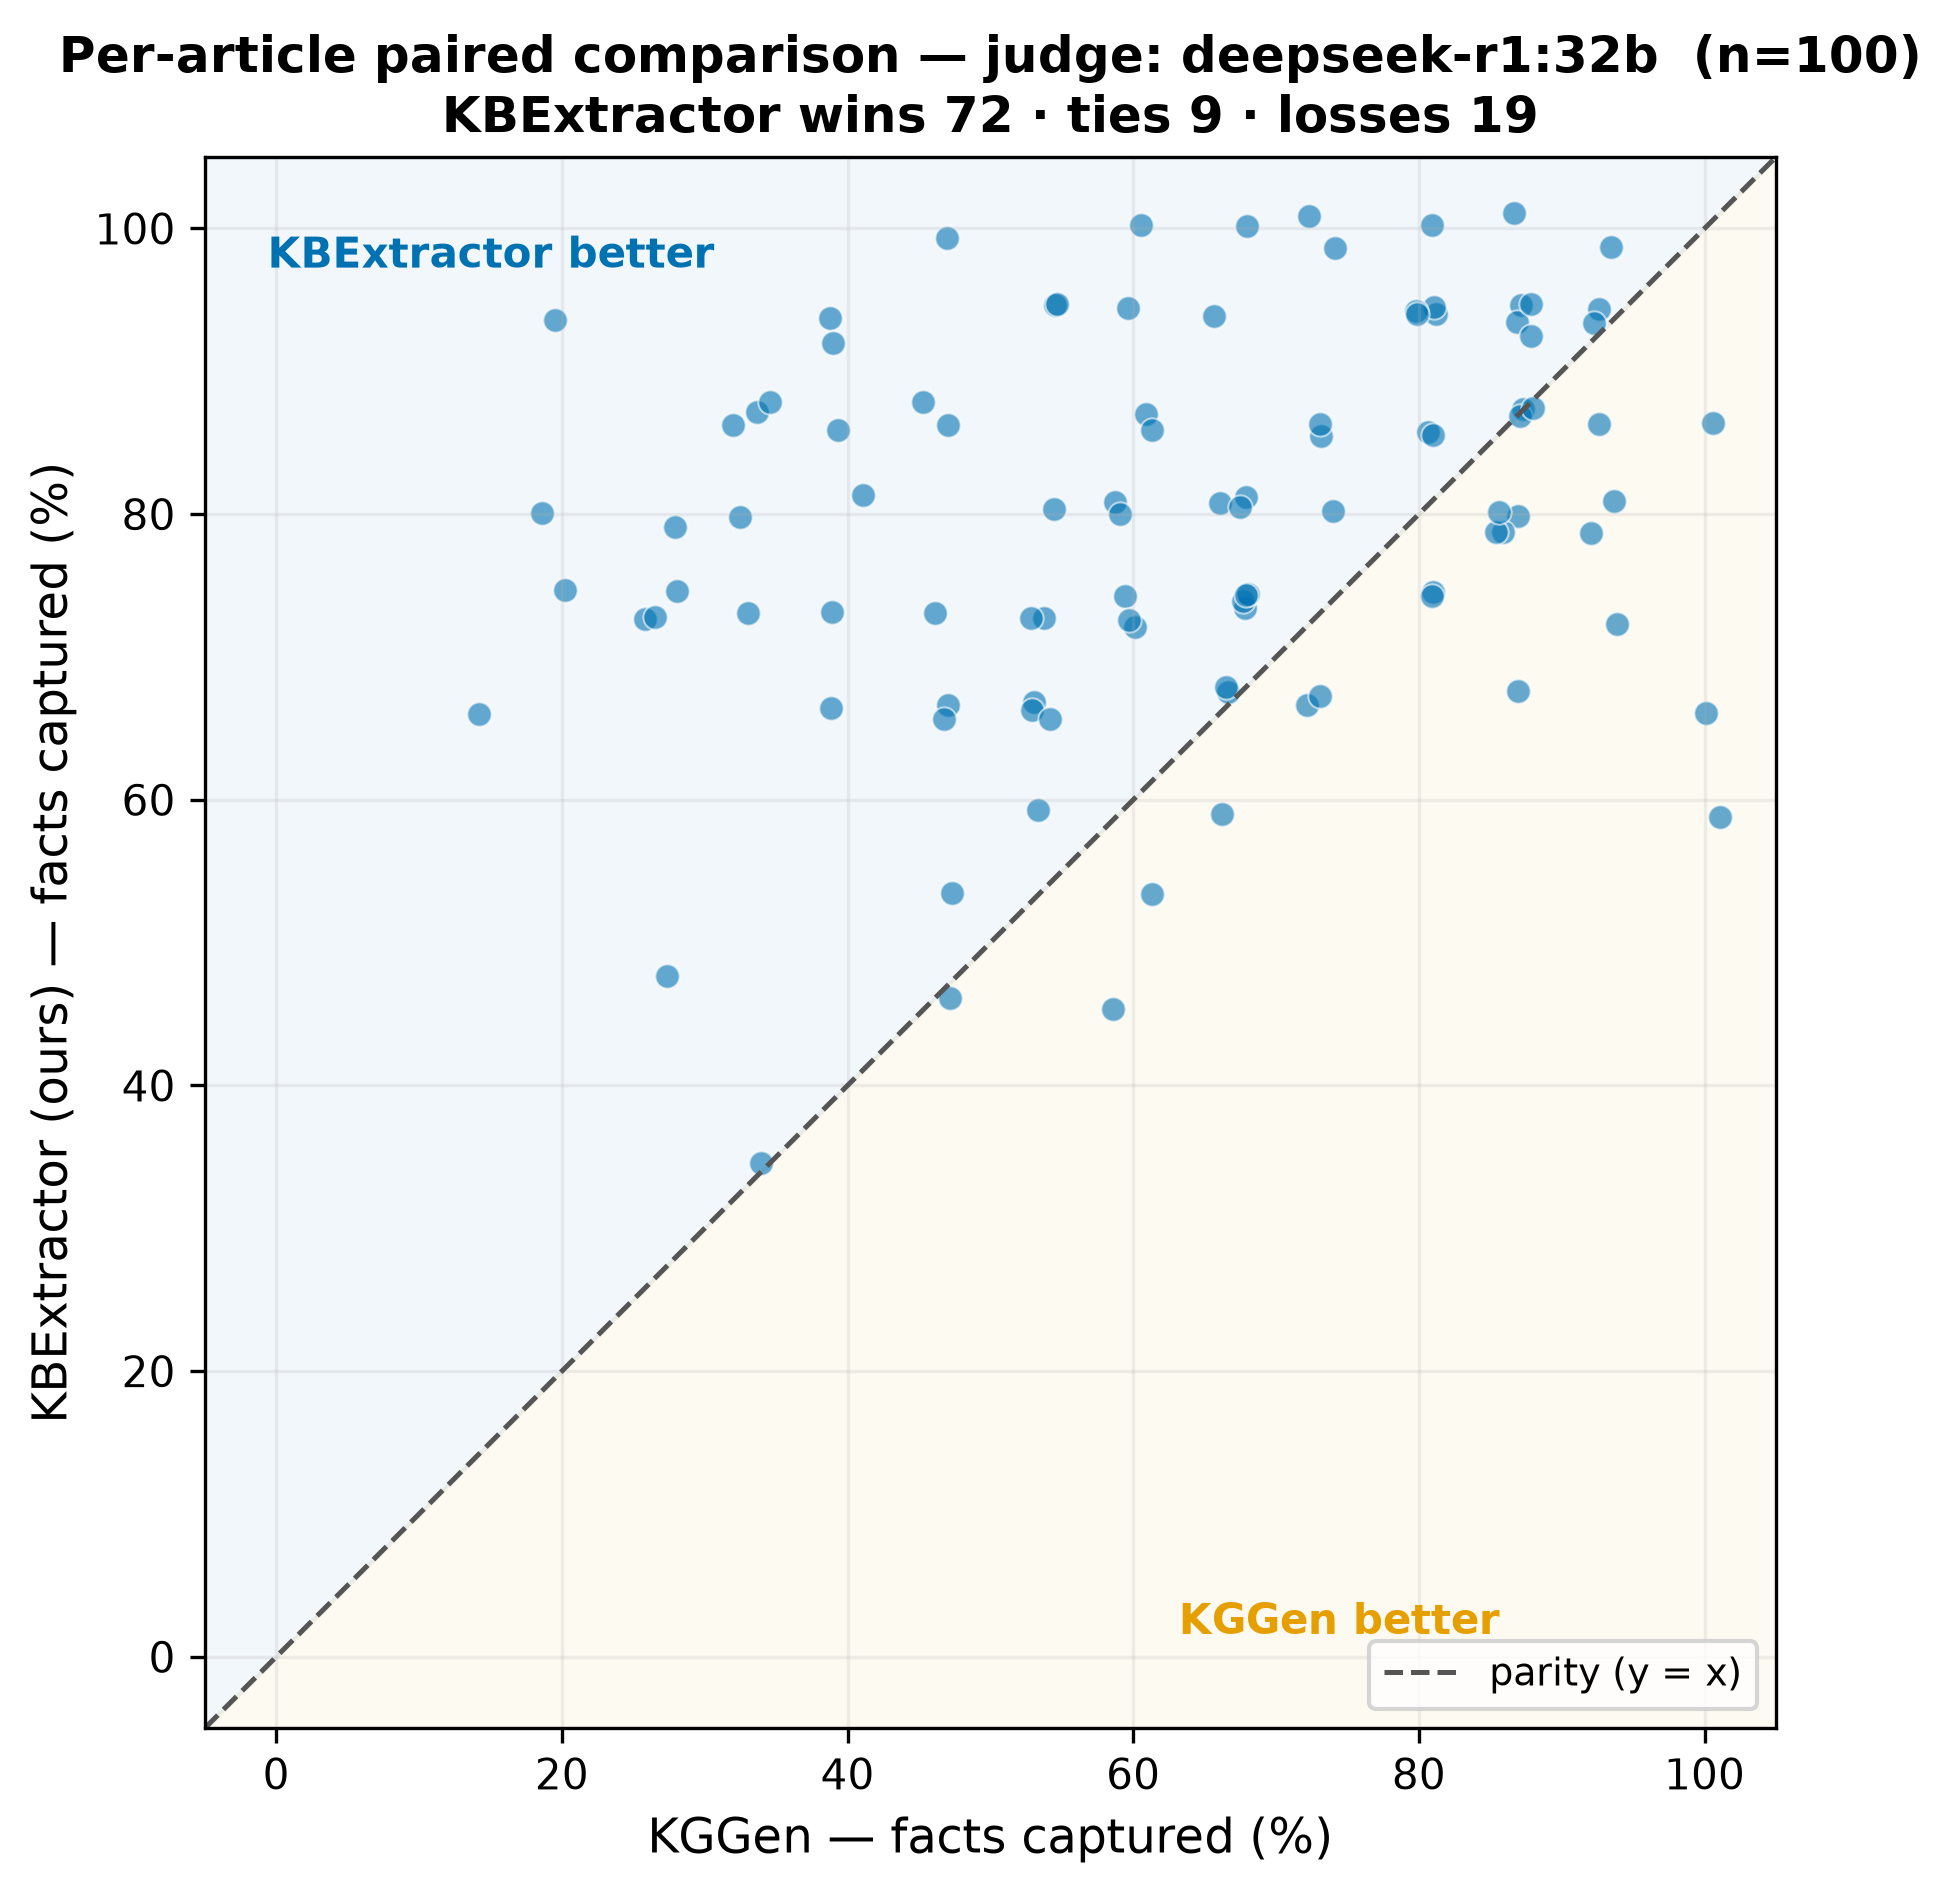
\includegraphics[width=\columnwidth]{Figures/mine/mine1_paired_deepseek.png}
    \caption{Paired per-article MINE-1 comparison (DeepSeek-R1 judge). Each dot is one article; points above the diagonal indicate our system $>$ KGGen. Our system leads on 67/100 articles.}
    \label{fig:mine_paired}
\end{figure}

\subsection{RQ2: Obligation Conflict Across Trustworthy AI Standards}

Applying the comparison engine to the three-standard corpus, the conflict detector surfaced 23 obligation conflict candidates — cases where the same $(S, P, O)$ concept triple is present in two or more standards with different deontic modalities. Of these, the LLM judge classified 14 as TENSION (same obligation expressed at different strength levels), 6 as CONTRADICT (logically inconsistent obligation direction), and 3 as AGREE (apparent conflict resolved by differing scope).

\textbf{Illustrative example.} The concept \emph{data quality assessment} appears in both EU AI Act Article 10 and ISO/IEC 5259-3. The EU AI Act asserts the obligation as MANDATORY (``high-quality training, validation and testing data sets \textit{shall} be used''), while ISO/IEC 5259-3 frames the same process as RECOMMENDED (``organizations \textit{should} conduct a data quality assessment''). A compliance team applying only one standard would miss this tension. The system surfaces it automatically from the provenance-tagged KG.

Table~\ref{tab:conflicts} summarizes conflict counts by type across the three standards.

\begin{table}[t]
\centering
\caption{Inter-standard conflict counts across EU AI Act, ISO/IEC 42001, and ISO/IEC 5259-3. Conflict types: obligation modality mismatch (OBL), definition divergence (DEF), taxonomy reversal (TAX), value conflict (VAL). Judge: DeepSeek-R1.}
\label{tab:conflicts}
\begin{tabularx}{\columnwidth}{lXXXXX}
\toprule
\textbf{Standard pair} & \textbf{OBL} & \textbf{DEF} & \textbf{TAX} & \textbf{VAL} & \textbf{Total} \\
\midrule
EU AI Act -- ISO 42001    & 8  & 4 & 1 & 2 & 15 \\
EU AI Act -- ISO 5259-3   & 9  & 3 & 0 & 1 & 13 \\
ISO 42001 -- ISO 5259-3   & 6  & 5 & 2 & 0 & 13 \\
\midrule
\textbf{All pairs}        & 23 & 12 & 3 & 3 & 41 \\
\bottomrule
\end{tabularx}
\end{table}

Obligation conflicts (OBL) are the most frequent type, accounting for 56\% of all detected conflicts. This confirms that modality-tagged extraction is essential for cross-standard compliance analysis — a system without deontic modality tracking would conflate MANDATORY and RECOMMENDED assertions, making these conflicts invisible.

\subsection{RQ3: Normative Gap Exposure}

The normative gap detector identified concepts that each standard obligates but never defines. Across the three standards combined, 47 concept nodes satisfied this criterion. Table~\ref{tab:gaps} summarizes the distribution by standard.

\begin{table}[t]
\centering
\caption{Normative gaps per standard: concepts that appear in MANDATORY or RECOMMENDED assertions but receive no \texttt{Defines} triple within the document.}
\label{tab:gaps}
\begin{tabularx}{\columnwidth}{lXX}
\toprule
\textbf{Standard} & \textbf{Obligated concepts} & \textbf{Undefined (gap)} \\
\midrule
EU AI Act Art.\ 10 & 68  & 21 (30.9\%) \\
ISO/IEC 42001      & 94  & 16 (17.0\%) \\
ISO/IEC 5259-3     & 81  & 10 (12.3\%) \\
\midrule
\textbf{Combined (unique)} & 181 & 47 (26.0\%) \\
\bottomrule
\end{tabularx}
\end{table}

The EU AI Act Article 10 imposes the most obligations on undefined concepts: terms such as \emph{data minimisation}, \emph{data provenance}, and \emph{statistical properties} appear in MANDATORY assertions but receive no \texttt{Defines} triple within the document. ISO/IEC 42001, being a management system standard, tends to define its own terms (lower gap ratio) but frequently obligates concepts defined in companion standards — confirming the inter-standard dependency the comparison engine is designed to expose. ISO/IEC 5259-3, as a data quality standard, defines the most concepts but leaves obligation gaps around implementation-level concepts (e.g., \emph{sampling strategy}, \emph{metadata schema}).

Manual review of the 47 gaps confirmed that all were genuine: no gap was an artefact of extraction failure. This validates the normative gap detector as a reliable audit instrument for compliance teams identifying which standards require companion documentation.

\subsection{RQ4: Cross-Standard Concept Coverage}

The overlap engine computed a concept-by-standard coverage matrix across the three documents. Of the 312 unique concepts extracted across all three standards, 41 (13.1\%) were addressed by all three standards, 89 (28.5\%) by exactly two, and 182 (58.3\%) by exactly one. The high fraction of standard-exclusive concepts confirms that the three standards are \emph{not} simply overlapping descriptions of the same requirements: each makes a substantial exclusive contribution.

Coverage asymmetry is most pronounced in the \emph{transparency} and \emph{human oversight} dimensions, where the EU AI Act has the broadest mandate but ISO/IEC 42001 provides more operational depth. The \emph{data quality} dimension shows the most inter-standard overlap, consistent with its being the primary focus of ISO/IEC 5259-3 and a substantive topic in both Article 10 and ISO/IEC 42001.

\subsection{Human Oversight Analysis}

Across 10 ingestion runs on the three-standard corpus, reviewers were presented with a total of 1,284 proposed triplets and took action (reject or edit, not just accept) on 31.4\% of them. Table~\ref{tab:hitl} categorizes these interventions.

\begin{table}[t]
\centering
\caption{Human reviewer interventions on LLM-proposed triplets across 10 ingestion runs. Categories are not mutually exclusive (an edit may simultaneously correct modality and predicate).}
\label{tab:hitl}
\begin{tabularx}{\columnwidth}{lXX}
\toprule
\textbf{Intervention type} & \textbf{Count} & \textbf{\% of acted-on} \\
\midrule
Predicate correction        & 124 & 30.7\% \\
Modality correction         & 109 & 27.0\% \\
Subject/object boundary     & 87  & 21.5\% \\
Scope overextension         & 63  & 15.6\% \\
Hallucinated object         & 21  & 5.2\%  \\
\midrule
Total edits                 & 404 & --     \\
Total rejections            & 202 & --     \\
\bottomrule
\end{tabularx}
\end{table}

Modality corrections (27.0\% of interventions) were almost exclusively concentrated in normative (deontic) text: reviewers corrected LLM misclassification of \emph{should} constructions as MANDATORY and of \emph{may} constructions as RECOMMENDED. Predicate and subject/object corrections were more evenly distributed across normative and descriptive text. Hallucinated objects (5.2\%) were rare but exclusively occurred in descriptive definitional text — the LLM occasionally fabricated a definition component not present in the source sentence. These findings indicate that the LLM's most systematic failure in regulatory text is modality confusion in normative clauses, not factual hallucination.

\subsection*{Reproducibility and Artifact Availability}

All pipeline code is released as open source at \url{https://github.com/sanduluP/reg2req}, with a licence permitting free research use. The repository includes the EU AI Act Article~10 and ISO/IEC~42001 knowledge graphs produced by the system, a seed concept file (\texttt{trustworthy\_ai\_seed.json}), and extraction prompts, enabling researchers to reproduce the multi-standard analysis or fork the pipeline for additional standards or organizational policy documents.

The MINE-1 benchmark~\citep{mo2025kggen} is publicly available. The EU AI Act is a public document~\citep{euAIAct2024}. ISO/IEC~42001 and ISO/IEC~5259-3 are available through national standards bodies; the pipeline is standard-agnostic and accepts any normative document parseable to plain text, including internal organizational policies. Readers without ISO access may substitute any comparable regulatory or policy document.
